% !TEX TS-program = pdflatex
% !TEX encoding = UTF-8 Unicode

\documentclass[11pt,a4paper]{book} % use larger type; default would be 10pt

\usepackage[utf8]{inputenc} % set input encoding (not needed with XeLaTeX)

%%% Examples of Article customizations
% These packages are optional, depending whether you want the features they provide.
% See the LaTeX Companion or other references for full information.

%%% PAGE DIMENSIONS
\usepackage{geometry} % to change the page dimensions
\geometry{a4paper} % or letterpaper (US) or a5paper or....
% \geometry{margin=2in} % for example, change the margins to 2 inches all round
% \geometry{landscape} % set up the page for landscape
%   read geometry.pdf for detailed page layout information

\usepackage{graphicx} % support the \includegraphics command and options

% \usepackage[parfill]{parskip} % Activate to begin paragraphs with an empty line rather than an indent

%%% PACKAGES
\usepackage{booktabs} % for much better looking tables
\usepackage{array} % for better arrays (eg matrices) in maths
\usepackage{paralist} % very flexible & customisable lists (eg. enumerate/itemize, etc.)
\usepackage{verbatim} % adds environment for commenting out blocks of text & for better verbatim
\usepackage{subfig} % make it possible to include more than one captioned figure/table in a single float
% These packages are all incorporated in the memoir class to one degree or another...

%%% HEADERS & FOOTERS
\usepackage{fancyhdr} % This should be set AFTER setting up the page geometry
\pagestyle{fancy} % options: empty , plain , fancy
\renewcommand{\headrulewidth}{0pt} % customise the layout...
\lhead{}\chead{}\rhead{}
\lfoot{}\cfoot{\thepage}\rfoot{}

%%% SECTION TITLE APPEARANCE
\usepackage{sectsty}
\allsectionsfont{\sffamily\mdseries\upshape} % (See the fntguide.pdf for font help)
% (This matches ConTeXt defaults)

%%% ToC (table of contents) APPEARANCE
\usepackage[nottoc,notlof,notlot]{tocbibind} % Put the bibliography in the ToC
\usepackage[titles,subfigure]{tocloft} % Alter the style of the Table of Contents
\renewcommand{\cftsecfont}{\rmfamily\mdseries\upshape}
\renewcommand{\cftsecpagefont}{\rmfamily\mdseries\upshape} % No bold!

\usepackage{hyperref} % om \url te kunnen gebruiken

\renewcommand\bibname{Resources} % Bibliography hernoemen

%%% END Article customizations

%%% The "real" document content comes below...

\title{Design and Development of Mass Expand, \\ a Bot for StarCraft: Brood War}
\author{Ben Haanstra, Armon Toubman}
%\date{} % Activate to display a given date or no date (if empty),
         % otherwise the current date is printed 

\begin{document}
\maketitle

\tableofcontents

\listoffigures

\listoftables

% Introduction
% !TEX root = report.tex

\chapter{Introduction}

In this report, we describe the design and development of a bot that plays the game StarCraft. A StarCraft bot is a computer program or script that plays a game of StarCraft. Our intention for the bot was to be capable of playing without any cheats, adapting to the state of the game and responding quickly. Although we initially pursued the goal of winning as well, we decided to change the focus on being capable of playing properly.

\section{The Game StarCraft}

StarCraft is a real-time strategy game developed by Blizzard and was shipped in 1998. Its foremost expansion Brood War was released later that same year. In general, when one talks about StarCraft, the expansion is implicitly included. Over the years, the game became quite popular as it introduced various interesting gameplay and multiplayer features that easily allowed for communities to grow.

There are three totally different races to be chosen from; the technologic advanced alien race Protoss with access to psionic weaponry and energy shields, the organic alien race Zerg that thrives on evolution and its great numbers to obliterate enemies, and the humanoid race Terran that focuses on conventional weaponry such as machine guns, tanks and nuclear weapons. Each of these races have their own unique units, structures, and their own unique style on how they should be played. In order to build and train those units, the resources Minerals and Vespene Gas have to be harvested and brought back to the main structure of the player.

The other reason that made StarCraft popular was that it is relatively easy to play online against others. This resulted in communities growing and many contests held, with large money prizes. Eventually, professional StarCraft player became a carreer for some. StarCraft was also one of the games used to pioneer \emph{Esports}, the digital variant of sports. In South Korea they showed matches live on television and developed large fanbases, players becoming celebrities, schools and training houses for teams were organized. With the fairly recent introduction of StarCraft II, however, the original game has decreased in popularity. Nevertheless, the game is still regarded as one of the best games made of all times.

The game also features an artificial intelligence, allowing players to try a \emph{skirmish} against the computer. The AI can play at four different levels, ranging from easy to insane, which was a new development at the time. But the AI itself was a very easily programmed script. It did not adapt to the players decisions, was quite repetitive and was easily misled. Furthermore, it cheats by having full observability over the whole field, while the game itself features a \emph{Fog of War} (areas out of sight range are blacked out). It also cheated by having unlimited resources, allowing it to train units even when being economically impaired.

%\begin{figure}
%\centering
%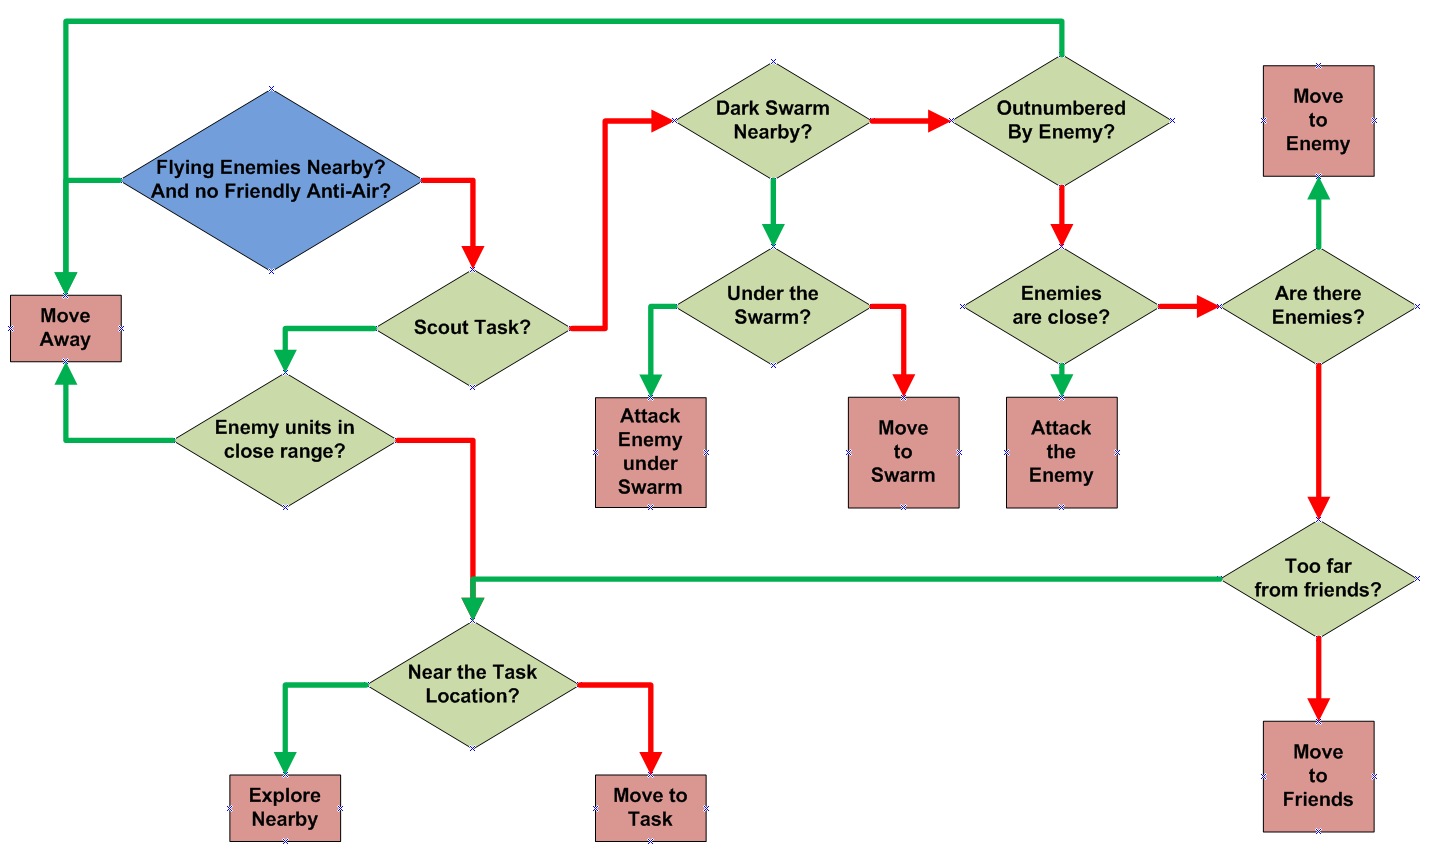
\includegraphics[scale=0.35]{starcraft_zerg_diagram_groot}
%\caption{\label{fig:micro} Flow chart illustration of the decision tree for 'Zergling' units. The blue rhombus is the start and is a decision node. Green rhombi are also decision nodes. Red squares are decision terminals that are to be executed. Green lines indicate a 'yes' answer to the respective question, and red lines indicate 'no'.}
%\end{figure}

\begin{figure}
        \begin{subfigure}[b]{0.5\textwidth}
                \centering
                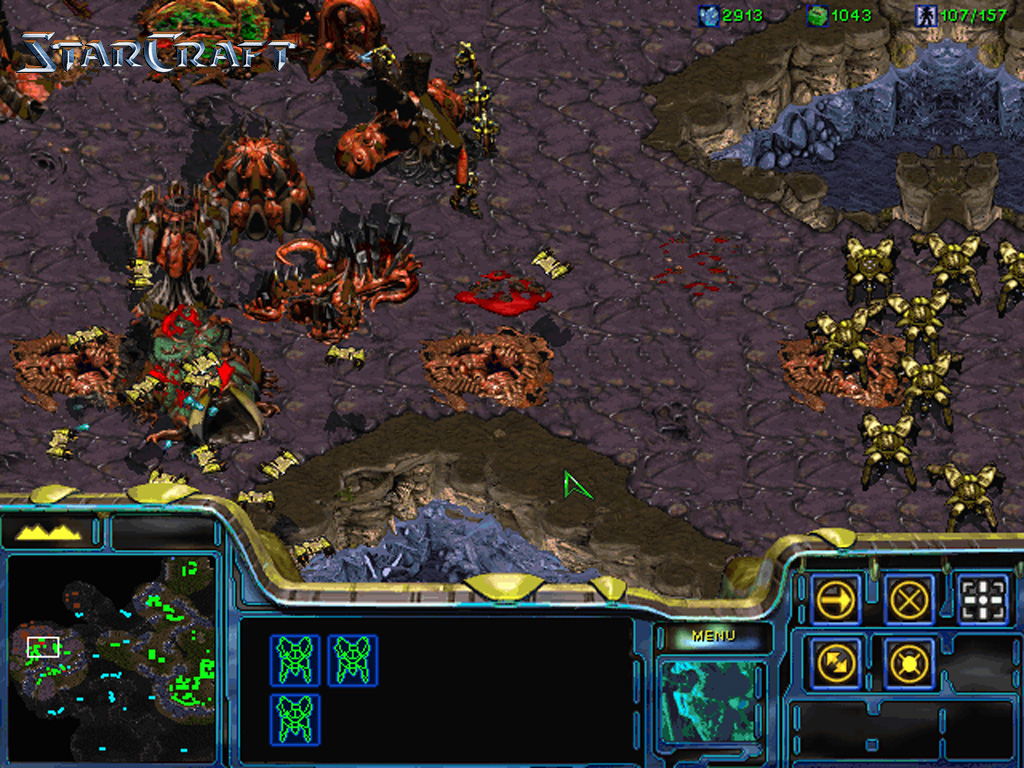
\includegraphics[width=\textwidth]{sc1}
        \end{subfigure}%
        ~ %add desired spacing between images, e. g. ~, \quad, \qquad etc. 
          %(or a blank line to force the subfigure onto a new line)
        \begin{subfigure}[b]{0.5\textwidth}
                \centering
                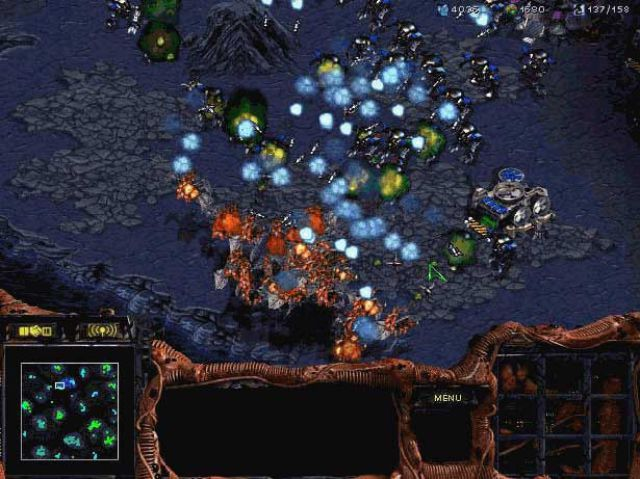
\includegraphics[width=\textwidth]{sc2}
        \end{subfigure}
        ~ %add desired spacing between images, e. g. ~, \quad, \qquad etc. 
          %(or a blank line to force the subfigure onto a new line)
        \caption{Images of battles in StarCraft Brood War}\label{fig:animals}
\end{figure}


\section{Goal of the Bot}
Our goal for the bot is to develop an AI that does not cheat and actually plays the game as it should. To make it more interesting than the standard AI already present in the game, we wanted something that could actually adapt to the playstyle of the opponent and also make its own strategies.

We arrived at this idea for a project when we stumbled upon an announcement for an AI competition for StarCraft, AIIDE2010, meant for bots to play each other. There were four different tournaments one could participate in, from very small scale battle to the complete game. The first two focused on team versus team battles. The third one is a simplified game of StarCraft, where both bots play Protoss, have only access to the units of the lowest tier of technology, and have to gather resources to produce units. The focus of this game is on a more strategic level, as units can not run quickly to the other side of the map. As for the fourth, we have a normal complete game of StarCraft. Although people were free to pick any race, it was adviced to program code for only one specific race. This is because StarCraft is a very detailed game and each race requires a complete different style.

Initially, we started out with the idea to win the competition, but quickly found out that there is a lot more to it than writing just code. Many teams of various universities signed up, some of them having more than 10 members. StarCraft is one of the most complex real-time strategies out there, and developing a very good bot involves a lot of knowledge of the game. Most of this knowledge is unfortunately unwritten and has to be accumulated by playing a lot of times. Knowledge on the top level, however, is prevalently available. For instance, what structures one should build to \emph{counter} the opponent's strategy, or what type of units are good against other type of units. In chapter \ref{chap:strategy}, we go into more detail on how we gathered knowledge.

As a result, we do not aspire to claim our bot is the best, but at least hope to make a versatile bot that can adapt and also initiate combat, without cheating. Furthermore, we wanted to participate in the AIIDE2010 competition's full game tournament, to see how well it works against other bots. As we neared completion of our bot, we decided to name it \massexpand{} referring to its tendency to create many additional bases.


\section{Outline of Report}
We first mention in chapter \ref{chap:libraries} the code made available and details of the competition. In chapter \ref{chap:strategy}, we describe our bot's structure abstractally; AI techniques considered, how units should behave, what overall decisions it has to make, and how we intent to achieve an autonomously adapative bot. The chapter \ref{chap:implementation} then goes into detail on how we implement our bot's strategy. Chapter \ref{chap:timeline} exhibits our timeline of the project and interesting events. We conclude this chapter in \ref{chap:conclusion}, where we also reflect on our choices.


%Many teams signed up, but at the submission deadline only about 30 teams were ready to participate. 





%We started out our project after we came across an Artificial Intelligence (AI) competition for the game; AI2010, a competition meant for bots playing against each other. In this competition, there were four tournaments one could participate in, each tournament having different rules or focus. The first two were focussed on how to control small groups of units, i.e. tactics on how units should work together locally.
%
%The third was a simplified game of StarCraft, were only units and structures of the lowest tier of technology were available. Here, the focus shifts more to placing units appropriately over the map. 
%%% We participate in the AI2010 competition

% Project goals (project voor vak, meedoen aan toernooi)

% Programming tools (bwapi/bwsal/bwta)

% Architecture (schema van geheel, beschrijving van alle onderdelen)

% Strategy
%    Micro
%    Bouwen

% Evaluation (testresultaten)

% Conclusion

% Resources (links naar source/docs/bwapi etc.)
% !TEX root = report.tex

\nocite{*}

\begin{thebibliography}{99}

\bibitem{massexpandproject}
	MassExpand project page.\\
	\url{http://code.google.com/p/massexpand/}

\bibitem{massexpanddocs}
	MassExpand code documentation.\\
	\url{http://www.armontoubman.com/massexpand/html/index.html}

\bibitem{starcraft}
	Blizzard Entertainment: StarCraft.\\
	\url{http://us.blizzard.com/en-us/games/sc/}

\bibitem{aiidecomp}
	AIIDE 2010 StarCraft AI Competition page.\\
	\url{http://eis.ucsc.edu/StarCraftAICompetition}

\bibitem{bwapi}
	BWAPI project page.\\
	\url{http://code.google.com/p/bwapi/}

\bibitem{bwsal}
	BWSAL project page.\\
	\url{http://code.google.com/p/bwsal/}

\bibitem{bwta}
	BWTA project page.\\
	\url{http://code.google.com/p/bwta/}

\bibitem{liquipedia}
	Liquipedia StarCraft Strategies \\
	\url{http://wiki.teamliquid.net/starcraft/Main_Page}

\bibitem{videos}
	Replay videos for knowledge elicitation: consulted YouTube channels and archives \\
	\url{http://eis.ucsc.edu/StarCraft_Data_Mining}\\
	\url{http://www.gosugamers.net/starcraft/replays/}\\
	\url{http://www.teamliquid.net/replay/}\\
	\url{http://www.youtube.com/user/ESportsTV}\\
	\url{http://www.youtube.com/user/nevake}\\
	\url{http://www.youtube.com/user/Jon747}\\
	\url{http://www.youtube.com/user/StarCraftLegacy}


\end{thebibliography}

\end{document}
